\documentclass{book}
\raggedbottom
\usepackage[a4paper,margin=1in]{geometry}
\usepackage{mdframed}
\usepackage{soul}
\usepackage{graphicx}
\usepackage[export]{adjustbox}
\graphicspath{{./images/}}
\usepackage{datetime}
\newdate{date}{02}{04}{2020}
\title{Mathematics Notes}
\author{Shyam S. Gupta}
\date{\displaydate{date}}
\begin{document}
	\maketitle
	\tableofcontents

	\chapter{Number Systems}
	\section{Introduction}
	\begin{itemize}
	\item \textbf{N, Natural Numbers}: 1,2,3...
	\item \textbf{W, Whole Numbers}: 0,1,2,3,...
	\item \textbf{Z, Integers}: ...-3,-2,-1,0,1,2,3,...
	\item \textbf{Q, Rational Numbers}
	\item \textbf{P, Irrational Numbers}
	\item \textbf{R (Real Numbers)}: Collection of all rational and irrational numbers, i.e. a real number is either rational or irrational.
	\end{itemize}
	
	\section{Real Number Line}
	\paragraph{Number Line}
	On the number line, distances from a fixed point are marked in equal units positively in one direction and negatively in the other . The point from which the distances are marked is called the \textbf{origin}. We use the number line to represent the numbers by marking points on a line at equal distances. If one unit distance represents the number 1, then 3 units distance represents the number 3, 0 being at the origin. The point in the positive direction at a distance $r$  from the origin represents the number r . The point in the negative direction at a distance r  from the origin represents the number $-r$.
	\paragraph{Real Number Line}
	Every real number is represented by a unique point on the number line. Also, every point on the number line represents a unique real number - this is why the number line is called the Real Number Line.
	
	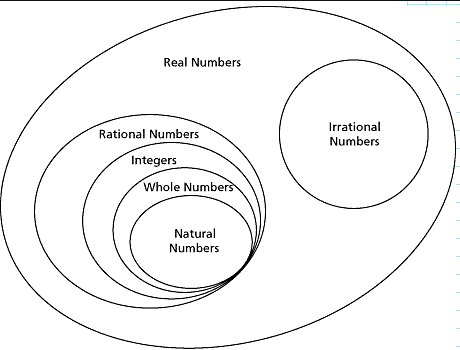
\includegraphics[scale=0.7]{numbersystem}
	
	\section{Rational Numbers}
	\textbf{Definition: }A number 'r' is called a rational number if it can be written in the form $p/q$, where:
	\begin{itemize}
	\item 	$p$ and $q$ are integers 
	\item $q \neq 0$
	\item $p$,$q$ have no common factors other than 1 (i.e. p and q are co-prime).
	\end{itemize}
	
	\underline{	\textbf{Important properties of Rational Numbers:}}
	\begin{itemize}
	\item An integer, for example $25$, can be written as $25/1$, therefore rational numbers include natural numbers, whole numbers and integers.
	\item Rational numbers do \textbf{NOT} have a unique representation in the form $p/q$. For example, $1/2 = 2/4 = 10/20$ and so on. These are \textbf{equivalent rational numbers}.  When we say $p/q$ is a rational number or represent it on the number line, we assume that $p$ and $q$ are co-prime. On the number line, among the infinitely many fractions equivalent to $1/2$, we will choose $1/2$ to represent them all.
	\item There are infinitely many rational numbers between any two given rational numbers.
	\item $0$ is a rational number
	\item Decimal expansion of a rational number is either terminating (example $1/4 = 0.25$) or non-terminating recurring (example $1/3 = 0.333.....$)
	\item Number of recurring entries is less than the divisor. For example, in $1/7$, there are six entries $326451$ in the repeating string of remainders and $7$ is the divisor. If the remainder's repeat, then we get a repeating block of digits in the quotient ($142857$ in case of $1/7$).
	\item If $x$ is a rational number (of the form $p/q$, where $p$ and $q$ are co-prime), whose decimal expansion terminates,  then prime factorization of $q$ is of the form $2^m5^n$, where $n$ and $m$ are non-negative numbers. Vice versa is also true, i.e. if prime factorization of  $q$ sis of the form $2^m5^n$, then $x$ has a decimal expansion which terminates. If the prime factorization of $q$  is not of the form $2^m5^n$ then the decimal expansion is non-terminating and recurring.
	\end{itemize}
	
	\section{Irrational Numbers}
	\begin{itemize}
	\item A number $s$ is called irrational, if it \textbf{cannot} be written in the form $p/q$, where p and q are integers and $q \neq 0$
	\item The decimal expansion of an irrational number is non-terminating and non-recurring.
	\end{itemize}
	
	\section{Examples}
	\begin{mdframed}[backgroundcolor=yellow]
		\textbf{Example: Express $0.333..$ as a rational number in the $p/q$ form.}
	\end{mdframed}
	\textbf{Solution:} \\
	$x = 0.333.....$ \\
	$10x = 3.333.... = 3 + 0.333... = 3 + x$ $=>$ $9x =3$ $=>$ $x=1/3$ \\
	
	\begin{mdframed}[backgroundcolor=yellow]
		\textbf{Example: Locate $\sqrt{3}$ on the number line}
	\end{mdframed}
	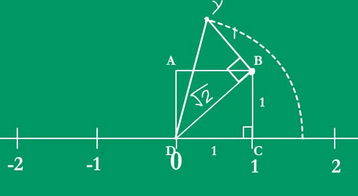
\includegraphics[scale=0.7]{squareroot} \\ \\
\textbf{Solution} \\ \\
Draw triangle $BCD$, where $BC=CD=1 => BD = \sqrt{2}$ \\
Draw $BY$ perpendicular to $DB$ , therefore $DY = \sqrt{3}$ \\
With center $D$ and radius $DY$ draw an arc intersecting the number line to locate $\sqrt{3}$ \\
Using this approach, you can locate the square root of other integers.
	\section{Square Root of Real Numbers}
If $a$ is a natural number, then $\sqrt{a} = b$ means $b^2 = a$ and $b>0$. In general, if $a>0$ be a real number and $n$ is a positive integer, then $\sqrt[n]{a} = b$ if $b^n =a$ and $b>0$. We follow the below convention:
\begin{mdframed} [backgroundcolor=yellow] 
	$\sqrt x$  represents the \textbf{positive square root} of $x$ and is called the  \textbf{principle square root } of $x$.
\end{mdframed}
For \textbf{$y=\sqrt[n]{x}$}:
\begin{table}[ht]

	\begin{tabular}{c c c c }
		\hline
		x & n & Result & Example \\
		\hline
		$x<0$ & $odd$ & There exists one negative $n^{th}$ root of $x$& $-2$ is the principle cube root of $-8$ \\
		$x<0$ & $even$ & $n^{th}$ root of $x$ is not a real number & $\sqrt{-16}$ is not Real
	\end{tabular}
\end{table}
\\
We must emphasize that \hl{$\sqrt{x^2} = \mid x \mid \neq x$}. For example, $\sqrt{-3^2} = \sqrt{9} = 3$ which is the absolute value of $\mid -3 \mid$.

	\section{Absolute Value}
	We now introduce the geometric concept of distance in the real number system. Let $a$ be the coordinate of a point on the number line - the number of units between this point and the origin $0$ is called the absolute value of $a$ and is denoted by \textbf{$\mid a \mid$} . Thus the absolute value of a number \textbf{gives only its distance from the origin and not its direction.}
	
	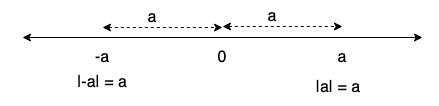
\includegraphics[scale=0.6]{absvalue} \\


In general,  if $a$ is any real number, then $\mid a \mid$ = $\mid -a \mid$, therefore the absolute value of a number is never negative. \\
Concept of absolute value can be used to measure the distance between two points - if $x_1$ and $x_2$ are coordinates for two points $A$ and $B$ on the real number line, then the distance between $A$ and $B$ is $\mid x_1 - x_2 \mid$ \\

\underline{\textbf{Important Propositions related to Absolute Value:}} \\

\begin{itemize}
	\item $\mid a \mid = \mid -a \mid$
	\item $\mid a.b \mid = \mid a \mid.\mid b \mid$
	\item $ab \leq \mid ab \mid$
	\item $\mid a+b \mid \leq \mid a \mid + \mid b \mid$
	\item $\mid a \mid - \mid b \mid \leq \mid a-b \mid$
	\item $\mid a/b \mid = \mid a \mid / \mid b \mid$
	\item $\mid \mid x \mid - \mid y \mid \mid \leq \mid x + y \mid \leq \mid x \ + \mid y \mid$
	\item $\mid x + y \mid = \mid x \mid + \mid y \mid$ when $x$ and $y$ have the same sign, i.e. $x.y \geq 0$
	\item Equations in absolute value must be equal to each other or be negative to each other. For example, if $\mid 3x +1\mid = \mid x-2 \mid $. This implies that $3x + 1 = x -2$ or $3x+1 = -(x-2)$ and the solutions are $x={-3/2,1/4}$
\end{itemize}

	\section{Intervals}
	\textbf{Open Interval}:  If $a$ and $b$ are real numbers and $a<b$,  then the open interval from $a$ to $b$ is written $(a,b)$ , is the collection of all real numbers greater than $a$ and less than $b$, i.e. $(a,b) = {{x | a<x<b}}$ . Geometrically, its represented on the real number line as shown below - the open circles represent the fact that $a$ and $b$ are \textbf{not included} in the interval. \\
	\\
	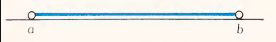
\includegraphics[scale=0.5]{openinterval}
	\\
	
	\textbf{Closed Interval}:  If $a$ and $b$ are real numbers and $a<b$,  then the closed interval from $a$ to $b$ is written $[a,b]$ , is the collection of all real numbers greater than equal to $a$ and less than equal to $b$, i.e. $[a,b] = {{x | a \leq x \leq b}}$ . Geometrically, its represented on the real number line as shown below - the closed circles represent the fact that $a$ and $b$ are also \textbf{included} in the interval. 	\\
	\\
	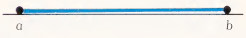
\includegraphics[scale=0.5]{closedinterval}
	
	\section{Euclid's Division Lemma}
	\begin{mdframed}[backgroundcolor=yellow]
		Given positive integers $a$ and $b$, there exist unique integers $q$ and $r$ satisfying $a = bq + r$ where $0 \leq r < b$
	\end{mdframed}
	
	\subsection{Highest Common Factor}
	HCF of two positive integers $a$ and $b$ is the largest positive integer $d$ that divides both $a$ and $b$. We can use Euclid’s division lemma to find the HCF of two positive integers. For example, to find the HCF of 455 and 42: \\
	1. Start with highest number, $455 = 42 \times 10 + 35$ \\
	2. Now consider the divisor and remainder: $42 = (35 \times 1) + 7$ \\
	3. Repeat the above step with divisor and remainder, $35 = (7 \times 5) + 0$\\
	4. Since the remainder is zero, the divisor at this stage, i..e $7$ will be the HCF \\
	
	\begin{mdframed}[backgroundcolor=yellow]
		$HCF(a,b) \times LCM (a,b) = a \times b$
	\end{mdframed}

	\section{Fundamental Theorem of Arithmetic}
	\begin{mdframed}[backgroundcolor=yellow]
		Every composite (i.e. non-prime) number can be factored as a product of primes, and this factorization is unique, apart from the order in which the prime factors occur.
	\end{mdframed}
	Example:  $32760 = 2^3 \times 3^2 \times 5 \times 7 \times 13$ \\
	\begin{itemize}
		\item $HFC(a,b)$  is the product of smallest power of each “common” prime factor. Example, $6 = 2^1 \times 3^1$ and $20 = 2^2 \times 5^1$ , so the HCF = $2^1$ which is the only common prime factor.
		\item $LCM(a,b)$ is the product of “greatest” power of “each” prime factor involved in the numbers. So in the above example, $LCM(6,20)$ will be $2^2 \times 3^1 \times 5^1 = 60$
	\end{itemize}

	\chapter{Polynomials}	
	
	\section{Introduction}
	Consider $-x^3 + 4x^2 +7x -2$
	\begin{itemize}
		\item \textbf{Terms}: This polynomial has four terms, $-x^3, 4x^3, 7x,-2$
		\item \textbf{Coefficient}: Coefficients of the four terms are $-1,4,7,-2$
		\item \textbf{Exponents should be whole numbers.} For exampple, $1 + 1/x$ is not a polynomial, as the coefficient of the second term is $-1$ which is nota whole number. Another example is $\sqrt{x} + 3$.
		\item \textbf{Constant Polynomial}: Example, $2$ is also a polynomial
		\item \textbf{Zero Polynomial}: Constant $0$ is called the zero polynomial
		\item \textbf{Monomial}: Polynomial with only one term
		\item \textbf{Binomial}: Polynomial with two terms
		\item \textbf{Degree of a polynomial}: Highest power of the variable in a polynomial. For example the degree of $-x^3 + 4x^2 + 7x + 2$ is $3$
		\item Degree of a non-zero constant polynomial is zero, degree of a zero polynomial is not defined
		\item \textbf{Linear Polynomial}: Degree is $1$. For example, $p(x) = 4x + 5$ is a linear polynomial and is of the form $ax + b$, can contain a maximum of two terms.
		\item \textbf{Quadratic Polynomial}: Degree is 2, is of the form $ax^2 + bx + c$ and will contain a maximum of three terms. In general, a polynomial of degree $n$ will contain a maximum of $n+1$ terms.
		\item \textbf{Zero of a Polynomial}: Consider $p(x) = x -1$. When we equate $p(x)$ to $0$, we get $x=1$, and $1$is the root (or zero) of the polynomial. 
		\item Non-zero constant polynomial has no zero
		\item Every real number is a zero of the zero polynomial
		\item A linear polynomial has one and only one zero \\
	\end{itemize}
In general, a polynomial on one variable $x$ of	degree $n$ is an expression of the form: \\
	\begin{mdframed}[backgroundcolor=yellow]
		$p(x) = a_nx^n + a_{n-1}x^{n-1} + ............ + a_1x + a_0$
	\end{mdframed}
where $a_0, a_1,...$ are constants and $a_n \neq 0$.
		
	\section{Remainder Theorem}
	If $p(x) $and $g(x)$ are two polynomials such that degree of $p(x)$ $>$ degree of $g(x)$ and $g(x) \neq 0$, then we can find polynomials $q(x)$ and $r(x)$ such that:
	
	$$p(x) = g(x)q(x) + r(x)$$ \\
	
where $r(x) =0$ or degree of $r(x)$ $<$ degree of $g(x)$. Essentially, what this means is $p(x)$ divided by $g(x)$ gives us $q(x)$ as the quotient and $r(x)$ as the remainder.
	\begin{mdframed}[backgroundcolor=yellow]
		\textbf{Remainder Theorem}:  Let $p(x)$ be any polynomial of degree $\ge 1$ and let $a$ be any real number. If $p(x)$ is divided by $x-a$, then the remainder is $p(a)$
	\end{mdframed}	

	\section{Factor Theorem}
	\begin{mdframed}[backgroundcolor=yellow]
		\textbf{Factor Theorem}:If p(x) is a polynomial of degree $n \ge 1$ and $a$ is any real number, then:
		\begin{itemize}
			\item $x-a$ is a factor of $p(x)$ if $p(a)=0$, and
			\item $p(a)=0$ if $x-a$ is a factor if $px$
		\end{itemize} 
	\end{mdframed}
	
	\section{Useful Identities}
	\begin{itemize}
		\item $(x+y)^3 = x^3 + y^3 + 3xy(x+y)$
		\item $(x-y)^3 = x^3 - y^3 -3xy(x-y)$
		\item $x^3 + y^3 + z^3 -3xyz = (x+y+z)(x^2 + y^2 + z^2 - xy -yz -zx)$
		\item $(x+y+z)^2 = x^2 + y^2 + z^2 + 2(xy + yz + zx)$
		\item $(x^3 + y^3)= (x+y)(x^2 -xy + y^2)$
		\item $x^3 - y^3 = (x-y)(x^2 + xy + y^2)$
	\end{itemize}
	\section{Synthetic Division}
	Synthetic division is used to divide one polynomial, $P(x)$ by a polynomial of the form $x-k$, where the coefficient of $x$ is $1$. It involves the below steps:
	\begin{enumerate}
		\item Arrange $P(x)$ in descending powers of $x$. If a term is missing, write a $0$ for its coefficient.
		\item Place $k$, the additive inverse of $-k$ in the divisor.
		\item Bring down the leading coefficient of largest power of $x$ to the 3rd row.
		\item Multiply the leading coefficient we bought down by $k$, place the product in the next position under the 2nd coefficient of the dividend and add the two numbers
		\item Multiply this sum by $k$, place the product under the 3rd coefficient and add.
		\item Continue this process until all coefficients in the dividend are used.
	\end{enumerate}

\begin{mdframed}[backgroundcolor=yellow]
	\textbf{Example: Divide $P(x) = 2x^4 - 3x^3 -4x + 8$ by $x-3$}
\end{mdframed}
\textbf{Solution: } : Using Synthetic Division, we can see from the below figure that the quotient is $2x^3 + 3x^2 + 9x + 23$ and remainder is $77$ \\

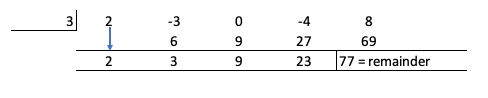
\includegraphics[scale=0.7, width=\linewidth, frame]{sdivision}

	\section{Zeros of a Polynomial}
	
	\begin{mdframed}[backgroundcolor=yellow]
		The zeros of a polynomial are the solutions to the equation $p(x) = 0$, where p(x) represents the polynomial. If we graph this polynomial as $y = p(x)$, then you can see that these are the values of $x$ where $y = 0$. In other words, they are the x-intercepts of the graph.
		\textbf{In general, given a polynomial $p(x)$ of degree $n$, will have a maximum of $n$ zeroes}
	\end{mdframed}

	\chapter{Graphs of Polynomial Functions}
	
	\section{Linear Polynomial - Straight Line}
	A linear polynomial is of the form $p(x) = mx + c$, and its graph is a straight line. Here $m$ is the slope or "steepness" of this straight line, i.e. how quickly it rises (or falls) as we move along the $x-axis$. The slope of a line is the ratio of $rise/run$:
	
	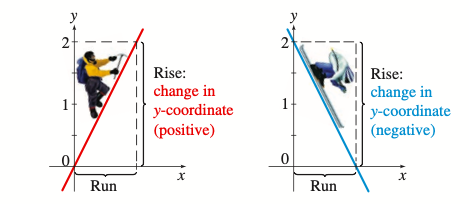
\includegraphics[scale=0.7]{slope1}

	The slope m of a nonvertical line that passes through the points $A(x_1,y_1)$ and $B(x_2,y_2)$ is
	
	$$m = rise/run = (y_2-y_1)/(x_2-x_1)$$
	
	\begin{itemize}
		\item A horizontal line has slope zero.
		\item The slope of a vertical line is not defined
		\item If two lines are parallel, they have the same slope
		\item If two lines are perpendicular to each other, the product of their slopes is $-1$
		\item Graph of $y = ax + b$ is a straight line which intersects the x-axis at exactly one point, $(-b/a,0)$. This means that a linear polynomial has exactly one zero, namely the point where the graph intersects the x-axis.
		\item Figure below shows several lines with their slopes - lines with positive slope slant upward to the right, whereas lines with negative slope slant downward to the right.
	\end{itemize}
	
	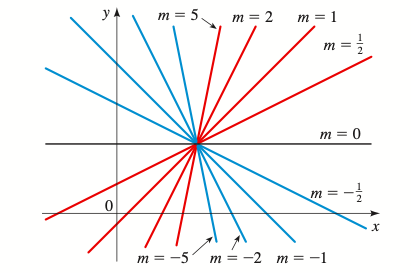
\includegraphics[scale=0.7]{slope2}
	
	\section{Quadratic Polynomial - Parabola}

	A quadratic polynomial can be written in the form $p(x) = ax^2 + bx + c$ where $a \neq 0 $ and $a,b,c$ are constants. \\
	The \textbf{standard form} of a quadratic function is $p(x) =a(x-h)^2 + k, a \neq 0$ \\
	The graph of a quadratic function is called a parabola
	\subsection{Leading Coefficient}
	\begin{itemize}
		\item In either form: If leading coefficient, $a>0$ then the parabola opens up. If leading coefficient, $a<0$ then the parabola opens down.
		\item The leading coefficient indicates how "fat" or how "skinny" the parabola will be:
		\begin{itemize}
			\item If  $\mid a \mid > 1$ the parabola will be "skinny" because it grows more quickly
			\item If $\mid a \mid < 1$,  the parabola will be "fat" because it grows more slowly.
		\end{itemize}
	\end{itemize}
	
	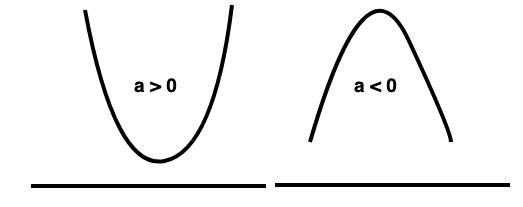
\includegraphics[scale=0.6]{parabolalc}
	
	\subsection{Vertex}
	The vertex is the lowest or highest point (depending on direction) on the graph of a quadratic function.
	\begin{itemize}
		\item In the non-standard form, i.e. $p(x) = ax^2 + bx + c$, the vertex is at the coordinate $-b/2a, p(-b/2a)$.
		\item In the standard form, $p(x) = a(x-h)^2 + k, a \neq 0$ the vertex is at the coordinate $(h,k)$.
		\item Let's assume we need to find the vertex of $p(x) = -(x-5)(x-9)$ which is in the factored form:
		\begin{enumerate}
			\item Determine the zeros, in this case it is $-2,4$
			\item Determine the x-coordinate of the vertex by averaging the zeros, $(-2+4)/2 = 1$
			\item Determine the y-coordinate of the vertex by substituting the x-coordinate of vertex and solving for y, $y = (1+2)(1-4)=-9$
			\item Vertex is (1,-9)
		\end{enumerate}
		
		
	\end{itemize}
	
	
	\subsection{Axis of Symmetry}
	Each parabola is symmetric about a vertical line called the axis of symmetry.  This vertical line goes through the vertex.
	\begin{itemize}
		\item In the non-standard form, i.e. $p(x) = ax^2 + bx + c$, the line of symmetry is represented by the vertical line $x= -b/2a$
		\item In the standard form, $p(x) = a(x-h)^2 + k, a \neq 0$ the line of symmetry is the vertical line $x = k$ 
		\item In the factored form, $p(x) = a(x-r_1)(x-r_2)$, the line of symmetry is the vertical line $x = (r_1 + r_2)/2$ 
	\end{itemize}
	
	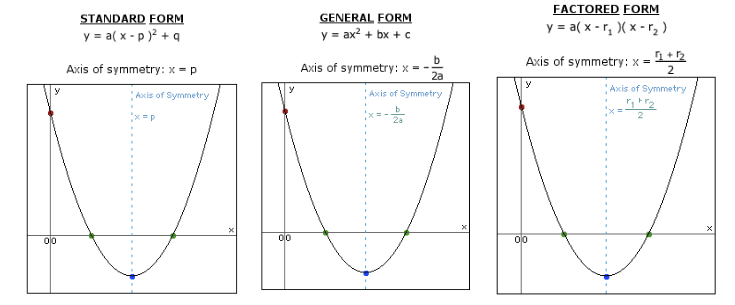
\includegraphics[scale=0.6]{parabolalos}
	
	\subsection{Discriminant}
	In the polynomial $p(x) = ax^2 + bx + c$, the $D = b^2 - 4ac$ is the discriminant.
	\begin{table}[ht]
		\begin{tabular}{|l| l| l|  }
			\hline
			\textbf{a} & \textbf{D} & \textbf{p(x)}\\
			\hline
			$a>0$ & $D<0$ & $p(x) >0 \forall x$\\
			\hline
			$a<0$ & $D<0$ & $p(x) >0 \forall x$\\
			\hline
			$a>0$ & $D=0$ & $p(x) >0 \forall x$ except at vertex.\\
			\hline
			$a>0$ & $D>0$ & $p(x)$ has two real roots $\alpha, \beta$, where $\alpha < \beta$. $p(x) > 0 \forall x \in (-\infty, \alpha) \cup (\beta, \infty)$. $p(x) < 0 \forall x \in (\alpha, \beta)$ \\
			\hline
			$a<0$ & $D=0$ & $p(x) < 0 \forall x$ except at the vertex \\
			\hline
			$a<0$ & $D>0$ &  $p(x)$ has two real roots $\alpha, \beta$, where $\alpha < \beta$. $p(x) < 0 \forall x \in (-\infty, \alpha) \cup (\beta, \infty)$. $p(x) > 0 \forall x \in (\alpha, \beta)$ \\
			\hline
		\end{tabular}
	\end{table}
	
	Please refer to the figure in the next page for the graphs associated with these conditions.
	
	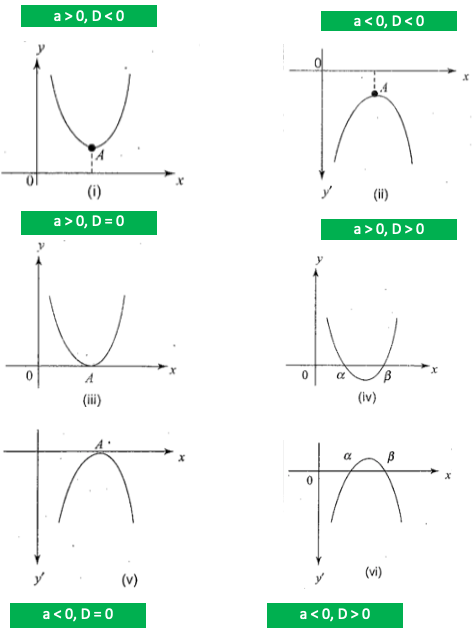
\includegraphics[scale=0.7]{parabolad} 
	
	\section{Graphs of Other Polynomial Functions}
	
	We will consider the polynomial function $p(x) = a_nx^n + a_{n-1}x^{n-1} + .....+ a_1x + a_0$, where $a_n \neq 0$ and the leading term is $a_nx^n$
	
	\subsection{Leading Coefficient and Degree}
	
	\begin{table}[ht]
		\begin{tabular}{|l| l| l|  }
			\hline
			\textbf{$n$} & \textbf{$a_n$} & Graph\\
			\hline
			Odd & Positive & Graph falls to the left and rises to the right\\
			\hline
			Odd & Negative & Graph rises to the left and falls to the right\\
			\hline
			Even & Positive & Graph rises to the left and to the right \\
			\hline
			Even& Negative & Graph falls to the left and to the right \\
			\hline
		\end{tabular}
	\end{table}

	Refer to the below figure for examples:-

	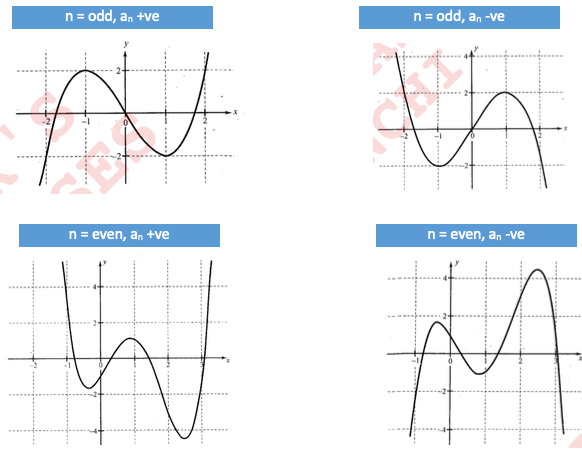
\includegraphics[scale=0.7]{polynomialg}
	
	\subsection{Zeroes and their multiplicities}
	A zero has a "multiplicity", which refers to the number of times that its associated factor appears in the polynomial. For example, consider the polynomial $p(x) = 3(x+5)^3(x+2)^4(x-1)^2)(x-5)$. The multiplicity of each zero is the number of times that its corresponding factor appears:
	
	\begin{itemize}
		\item $x=-5$ has an odd multiplicty of 3
		\item $x=-2$ has an even multiplicity of 4
		\item $x=1$ has an even multiplicity of 2
		\item $x=5$ has an odd multiplicity of 1
	\end{itemize}
	
	The point of multiplicities with respect to graphing is that any factors that occur an even number of times are squares, so they don't change sign. Squares are always positive. This means that the x-intercept corresponding to an even-multiplicity zero can't cross the x-axis, because the zero can't cause the graph to change sign from positive (above the x-axis) to negative (below the x-axis), or vice versa.  An even-multiplicity zero makes the graph just barely touch the x-axis, and then turns it back around the way it came. \hl{This means that the sign of $p(x)$ does not change on either side of zero with even multiplicity.}
	
	\begin{itemize}
		\item Any zero whose corresponding factor occurs in pairs (so two times, or four times, or six times, etc) will "bounce off" the x-axis and return the way it came. \item Any zero whose corresponding factor occurs an odd number of times (so once, or three times, or five times, etc) will cross the x-axis. 
	\end{itemize}
	
	Polynomial zeroes with even and odd multiplicities will always behave in this way. In the below figures, we can see that all  four graphs have the same zeroes, at x = –6 and at x = 7, but the multiplicity of the zero determines whether the graph crosses the x-axis at that zero or if it instead turns back the way it came. If the zero was of multiplicity 1, the graph crossed the x-axis at the zero; if the zero was of multiplicity 2, the graph just "kissed" the x-axis before heading back the way it came.
	
	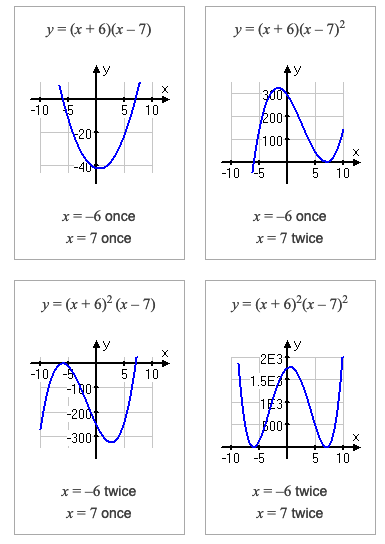
\includegraphics[scale=0.7]{zerom}
	
	\subsection{Turning Points}
	From the previous subsection we can see that the graph of a polynomial consists of a smooth line with a series of hills and valleys called turning points. 
	\begin{itemize}
		\item The maximum number of turning points is one less than the degree of the polynomial
		\item The point where the graph has a turning point, the derivative of the function/polynomial (i.e tangent/slope at that point will be parallel to x-axis) becomes zero, which provides the point of local minima or maxima.
	\end{itemize}
	
	Consider the below graph for example
	
	\begin{itemize}
		
		\item Tangent to the curve at point for which $x < -1$ and $x > 1$ makes an acute angle with the positive direction of x-axis, hence derivative is positive for these points.
		\item For $-1 < x < 1$, tangent to the curve makes an obtuse angle with the positive direction of x-axis, hence derivative is negative at these points.
		\item At $x=1$ and $x=-1$, the tangent is parallel to x-axis, where derivative is zero.
	\end{itemize}
	
	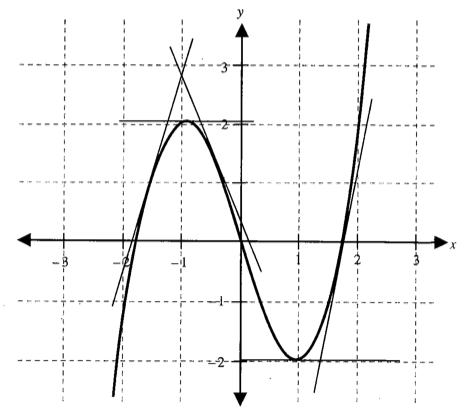
\includegraphics[scale=0.7]{turningpoint}
	
	\subsection{Positive and Negative Intervals}
	\hl{The sign of a polynomial between any two \textbf{consecutive zeros} is either always positive or always negative}. This is because polynomial functions are continuous functions (no breaks in the graph), which means that the only way to change signs is to cross the x-axis. But if this happened, the given zeros would not be consecutive! It is not necessary, however, for a polynomial function to change signs between zeros.
	\\
	
	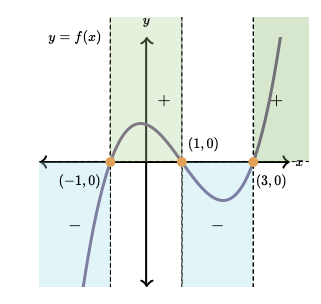
\includegraphics[scale=0.5]{pinterval1}
	
	Let's consider the polynomial $p(x) = (x+3)(x-1)^2$. The zeros are $-3,1$. This creates three intervals over which the sign of $p(x)$ is constant:
	\\
	
	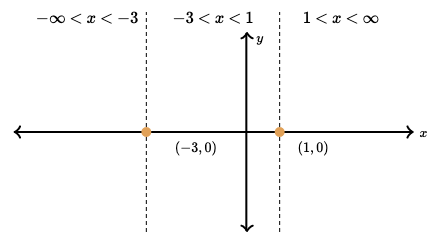
\includegraphics[scale=0.5]{pinterval2}
	
	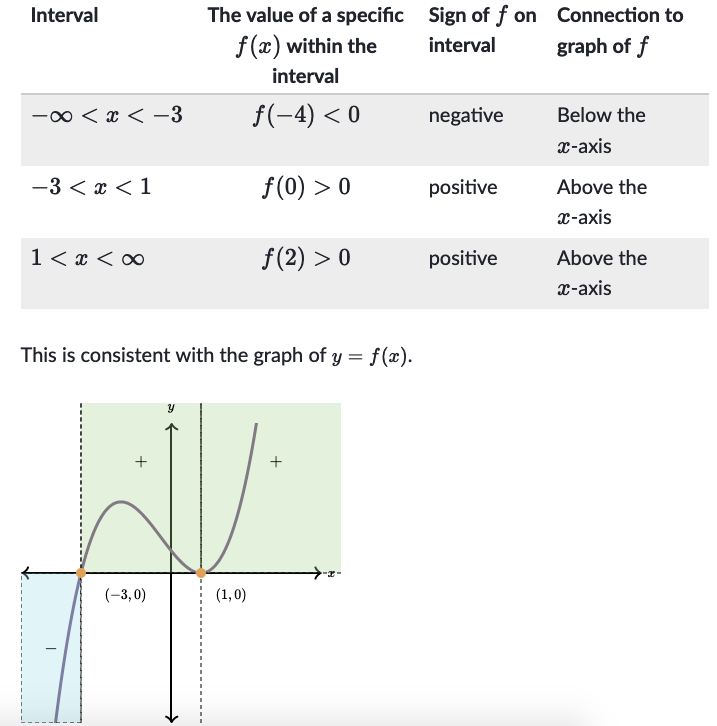
\includegraphics[scale=0.6]{pinterval3}
	
	\chapter{Quadratic Equations}
	
	\section{Introduction}
	When a quadratic polynomial, $p(x) = ax^2 + bx + c$ is equated to zero, we get a quadratic equation. Therefore, a quadratic equation is of the form $ax^2 + bx + c = 0$ where $a,b,c$ are Real Numbers and $a \neq 0$. \\
	$b^2 -4ac$ is called the Discriminant(D):
	\begin{itemize}
		\item If $D \ge 0$ then the roots are real, ${(-b \pm \sqrt{D})}/2a$
		\item If $D=0$, then we have two equal roots, $-b/2a$
		\item If $D<0$, then there are no real roots and the graph \textbf{does not} cut the x-axis.
		\item If $D>0$, then there are two \textbf{distinct} real roots and the graph will cut the x-axis at two places.
	\end{itemize}
	
	When coefficients $a,b,c$ are rational or integers:
	\begin{itemize}
		\item $D>0$ and its a perfect square: Roots are rational.
		\item $D>0$ and an imperfect square: Roots are irrational and exist as \textbf{conjugate pairs}.
	\end{itemize}
	
	\begin{mdframed}[backgroundcolor=yellow]
		Note 1: If $\alpha, \beta$ are the roots of a quadratic equation, then the equation can be written in the following ways:
		\begin{itemize}
			\item $(x - \alpha)(x - \beta) = 0$ (by factor theorem)
			\item $x^2 - (\alpha + \beta)x + \alpha\beta$ : This is useful when we know the sum and product of roots.
		\end{itemize}
	\end{mdframed}
	\begin{mdframed}[backgroundcolor=yellow]
		Note 2: If $\alpha, \beta$ are the roots of $ax^2 + bx + c = 0$, then:
		\begin{itemize}
			\item Sum of Roots, $\alpha + \beta = {(-b/2a)}$
			\item Product of Roots: $\alpha\beta = c/a$
		\end{itemize}
	\end{mdframed}
	
	\section{Common Roots}
	Let's consider the following quadratic equations:
	$$a_1x^2 + b_1x + c_1 = 0$$
	$$a_2x^2 + b_2x + c_2 = 0$$
	
	\subsection{Condition for one common root}
	If $\alpha$ is the common root for the above equations, then:
	$$a_1\alpha^2 + b_1\alpha + c_1 = 0$$
	$$a_2\alpha^2 + b_2\alpha + c_2 = 0$$
	
	Solving these two equations by cross-multiplication, we get the condition for one common root
	
	\begin{mdframed}[backgroundcolor=yellow]
		$$\alpha^2 / {(b_1c_2 - b_2c_1)} = \alpha/{(c_1a_2-c_2a_1) = 1/{(a_1b_2 - a_2b_1)}}$$
	\end{mdframed}
	
	\subsection{Condition for both roots to be common}
	Let $\alpha, \beta$ be the roots common to the above equation, which means that both equations are identical - the condition for this is:
	
	\begin{mdframed}[backgroundcolor=yellow]
		$$a_1/a_2 = b_1/b_2 = c_1/c_2$$
	\end{mdframed}
	
	\section{Location of Roots}
	For a given quadratic equation $ax^2 + bx + c = 0$, where $a>0$, the Discriminant(D) = $b^2-4ac$, we can have the following conditions:
	\subsection{Both roots are greater than a number $d$}
	All the conditions below must be true  for both roots $\alpha, \beta$ to be greater than a number $d$:
	\begin{itemize}
		\item $D>0$
		\item Line of Symmetry, $-b/2a > d$
		\item Value of $f(x) = ax^2 + bx + c$ at $d$ will be greater than $0$ 
	\end{itemize}
	
	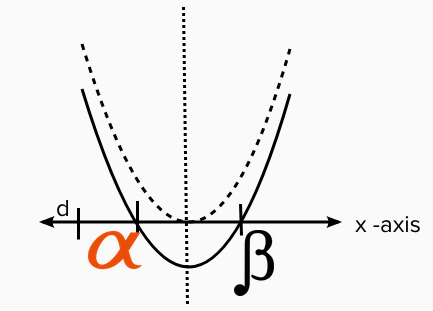
\includegraphics[scale=0.6]{condition1}
	
	\subsection{Both roots lie on opposite sides of a number $d$}
	In this case we cannot comment on the line of symmetry, which can lie on either side of $d$. Below conditions must be true:
	\begin{itemize}
		\item $D>0$
		\item Value of $f(x) = ax^2 +bx + c$ at $d$ is less than $0$.
	\end{itemize}
	
	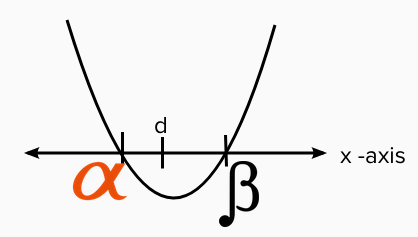
\includegraphics[scale=0.6]{condition2}
	
	\subsection{Both roots lie between $(d,e)$}
	\begin{itemize}
		\item $D>0$
		\item Line of Symmetry, $d < -b/2a < e$
		\item Value of $f(x) = ax^2 + bx + c$ at $d$ and $e$ is greater than zero.
		
		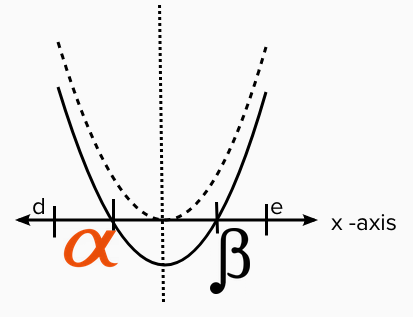
\includegraphics[scale=0.6]{condition3}
	\end{itemize}
	
	\subsection{$(d,e)$ lie between the roots}
	\begin{itemize}
		\item Value of $f(x) = ax^2 + bx + c$ at
		/\ $d$ and $e$ is less than zero.
	\end{itemize}
	
	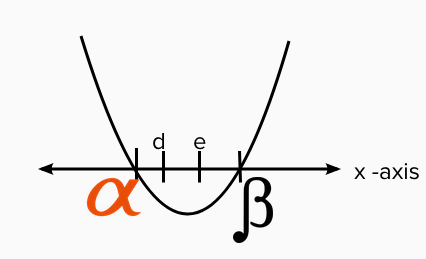
\includegraphics[scale=0.6]{condition4}
	
	\subsection{Exactly one root lies in interval $(d,e)$}
	\begin{itemize}
		\item $f(d)f(e) <0$, where $f(d),f(e)$ are values of $f(x) = ax^2+bx+c$ at $d,e$
		\item $f(d)f(e)=0$ - In this case, verify for extraneous roots that are not applicable
	\end{itemize}
	
	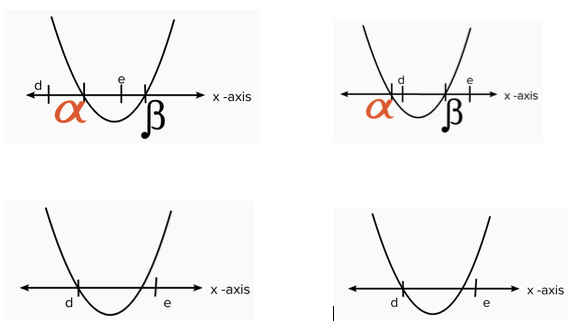
\includegraphics[scale=0.6]{condition5}
	
	\chapter{Logarithms}
	\section{Introduction}
	Exponent Form: $6^2 = 36$ \\
	Logarithmic Form: $log_6{36} = 2$
	\begin{mdframed}[backgroundcolor=yellow]
		In general, $log_aN = x$, where:
		\begin{itemize}
			\item Base $a>0$
			\item Base, $a \neq 1$
			\item $N > 0$ and $N \in R^+$, i.e. $N$ is a positive real number
		\end{itemize}
	\end{mdframed}
	\section{Identities}
	
	\begin{itemize}
		\item $log_NN = 1$
		\item In $log_aN$, if $a \times N =1$, (i.e. if $a$ and $N$ are reciprocal to each other) then it means that $logaN = -1$ 
		\item $log_a1 = 0$
		\item $log_aN + log_aM = log_a{NM}$
		\item $log_aN - log_aM = log_a{(N/M)}$
		\item $log_aN^\beta = \beta log_aN$
		\item$x^{log_xN} = N$
		\item $\ln x = log_ex$ , Natural Logarithm (Base $e$). The number $e$ is defined as the value that $(1 + 1/n)^n$ approaches as $n$ becomes large. The approximate value of $e$ is $2.718$,and it's an irrational number.
		\item $\ln x = y \leftrightarrow e^x = y$
		\item $log_{10}x$ , Common Log (Base $10$)
	\end{itemize}
	
	Here is the graph of $log_2x$: 
	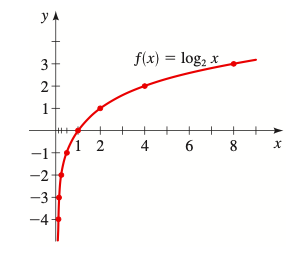
\includegraphics[scale=0.6]{loggraph}

	\chapter{Exponential Functions}
	
	\section{Introduction}
	\begin{mdframed}[backgroundcolor=yellow]
		An exponential function with base $a$ is defined for all real numbers $x$ by $f(x) = a^x$ where $a>0$ and $a \neq 1$
	\end{mdframed}
	
	\section{Graphs of Exponential Functions}
	 Figure below shows the graphs of the family of exponential functions $f(x) = a^x$ for various values of the base $a$. All of these graphs pass through the point $(0,1)$ because $a^0 = 1$ for $a \neq 1$.
	 
	 \begin{itemize}
	 	\item If $0<a<1$, the exponential function \textbf{decreases} rapidly.
	 	\item If $a>1$, the exponential function \textbf{increases} rapidly.
	 \end{itemize}
	 
	 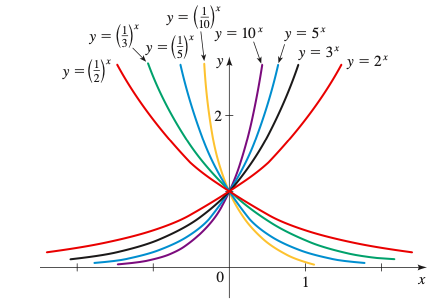
\includegraphics[scale=1.0]{expgraph}
	
	\section{Transformation of Exponential Functions}
	 \subsection{$f(x)=1+a^x$}
	 To obtain the graph of $1+a^x$, we start with the graph of $f(x) = a^x$ and shift it upward 1 unit.
	 
	 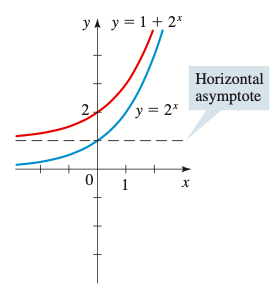
\includegraphics[scale=0.8]{exp1}
	 
	 \subsection{$f(x) = -a^x$}
	 We start with the graph of $f(x) = a^x$, but here we reflect in the x-axis
	 
	 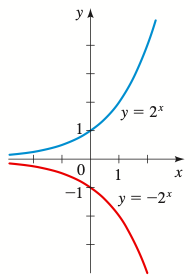
\includegraphics[scale=0.8]{exp2}
	 
	 \subsection{$f(x) = a^{-x}$}
	 In this case, the graph is the mirror image of $f(x) = a^x$
	 
	 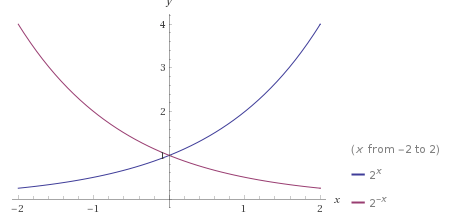
\includegraphics[scale=0.8]{exp3}
	 
	 \section{The Natural Exponential Function}
	 The number $e$ is defined as the value that $(1+1/n)^n$ approaches as $n$ becomes large. The approximate value is $e = 2.71828$. The number $e$ is the base for natural exponential function, which in certain applications is easier to work with than $log_{10}$. \\
	 The \textbf{natural exponential function} is the function $f(x) = e^x$ with base $e$. Since $2 < e < 3$, the graph of $e^x$ lies between the graphs of $2^x$ and $3^x$:\\
	 \\
	 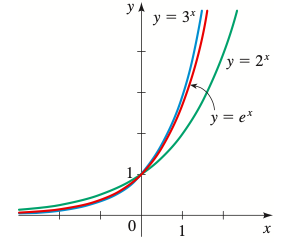
\includegraphics[scale=0.8]{exp4}
	
\end{document}